

\documentclass{article}
\usepackage{blindtext}
\usepackage[utf8]{inputenc}
\usepackage{graphicx}
\usepackage{placeins}
\graphicspath{{images/}}
 
\title{Topic Modelling in Twitter – approaches old and new}
\author{Kristy James}
\date{\today}
 
\begin{document}
 
\maketitle
 
\section{Introduction}

 Although the motivations of the original research articles replicated here were to improve the state of the field of language modelling in general (by, for instance, creating interpolated models with the best performance on concrete tasks such as speech recognition, or by measuring perplexity over a test corpus), this paper does not attempt to construct a full model (eg by interpolating with a standard trigram model). Rather, the aim is to compare the topic-associations that each of these approaches was able to mine from the data. 
[something snappy]

The first section of this paper outlines the motivation for topic-modelling over a micro-blog corpus, drawing examples from recent literature where real-world applications used these models, and discussing the state-of-the-art techniques. Thereafter follows an explanation of the corpus used for the training and evaluation of these models, a subset of the RUG’s Dutch Twitter corpus, and how the nature of micro-blogs influences assumptions made for testing (eg. how the data was split, which days the data was collected on, etc).

The third section describes the topic-modelling approaches tested in this paper, outlining the theory behind these approaches and assumptions made for this experiment.

The fourth section describes previous work that considered how best to evaluate topic-clusters, and …

Following this are the results of the experiment and a discussion…


 
\section{Motivation}

TODO: Why document clustering is different to the traditional clustering in LMs
 
Topic identification of tweets has been conducted for many purposes:
Ramage, Dumais and Liebling aim to optimize user's experience with their twitter feed by hiding posts about irrelevant topics, whereas other topic model variations have real-time first story detection (Lau et al), user-recommendation () or event-related burst detection () as their aim. Famously, topic modeling on twitter has been used to measure flu (), protests () and detect crime(Wang et al 2012).
Aside from collaborative filtering for online topic detection, (Diaz-Alvires et al 2012, find some more alternative methods), hybrid systems, including sytactic filtering, duplicate detection and set theory heuristics (O'Connor, Krieger and Ahn, XXXX), have been used for this task.

Recently, Latent Dirichlet Allocation (Blei et al, year) has emerged as the most popular tool for unsupervised learning of topic associations of documents, particularly micro-blogs.
However, one parameter that is calculated in LDA is the assignment of theta ~ Dir(alpha), namely the probability distribution describing the contribution of each topic to the document, which depends on the choice of alpha, the number of topics that each document can maximally be assigned to. An assumption that could be made about the majority of micro-blog posts, given their short nature, is that they in general only handle one topic (depending, of course, on the granularity of the topic distinctions). Also, as the ultimate goal in this situation is to build a language model that does not have too many zero-occurrences of relevant words, the topics must by nature be broad enough to be useful, ensuring that if the topic granularity is chosen correctly, then most micro-blogs will cover one topic (as relevant for language modelling purposes, this does not intend to put forward a thesis of a semantic nature).

Additionally, sentence-mixture language models (Iyer and Ostendorf, 1999) also allow for dynamic adaptation using a cache, so that words already mentioned in a document (per topic) are assigned extra probability due to the fact of them being mentioned already. It is easy to see that the application of a cache language model to micro-blogs would be frivolous, because in a short text it is unlikely for the authors to waste space repeating themselves. However, if the topic groupings of tweets can be reliably captured, a topic-wide cache language model can be maintained, monitoring not an individual's use, rather the platform-wide discourse, or the trending subjects within a topic.

With far less lofty aims, this paper explores two disparate aims:
\begin{enumerate}
	\item Improve user experience of the twitter mobile interface by:
	\begin{enumerate}
		\item improving the language model used in the typing interface, by guessing the topic of the post and thus being able to:
		\item include trending topic-specific words
		\item suggest relevant (trending) hashtags that will allow for greater public engagement with their post for people outside their immediate network (		This is a relevant aim because twitter is widely used as a mobile application [find some stats], where the user may not have access to a traditional keyboard. Language models are essential for autocorrect functions, and can be frustrating when they return outdated suggestions.)
		\item Note: Weng made a topic model based on users' messages, see more about this
	\end{enumerate}
	\item As a comparison to LDA, investigate alternative unsupervised 'bag-of-words' topic-elicitation techniques which are then used to construct language models, comparing their efficacy and their efficiency.  These can be broadly grouped into two types, those which assign each document to only one cluster (hard clustering) and those which return the probability that a document belongs to a particular cluster (soft clustering).
\end{enumerate}
 
 \begin{center}
 	\begin{table}
 	\begin{tabular}{|p{3cm}|p{8cm}|}
 		\hline
 		Hard Clustering &  Flat clustering minimizing unigram perplexity (Goodman 2001); Agglommerative clustering based on tf.idf-like scoring (Iyer and Ostendorf 1999); kMeans based on tf.idf  \\
		\hline
 		Soft Clustering &  Latent Dirichlet Allocation (reference); Latent Semantic Analysis (reference); Building Topic-LMs with EM (Iyer and Ostendorf 1999, second step); Topic-based Language Models with EM (Gildea and Hoffman, 1999) \\
 		\hline	
 	\end{tabular}
	\caption{Methods of eleciting topics explored.}	
 	\end{table}
 \end{center}
 
 In the case of the hard-clustering methods, the topics are first determined with one kind of language model, and finally, once the clusters are set, a full language model (eg trigram) is built over the documents in the cluster. In the soft-clustering methods, however, the methods return language models for each topic, as well as the probability with which each document represents each topic. For visualisation purposes, the largest document prior is deemed the cluster it is assigned to, though in reality the assignment of the training documents to clusters is immaterial to the performance of the language models derived from them.
The above-mentioned methods are not often implemented for twitter-based tasks, given that LDA is the most common technique applied, and indeed very successfully. Thus the contribution of this paper is to explore

% Evaluation methods of LSA have been discussed (Wallach et al, 2009), as well as methods for choosing the optimal number of topic mixtures for a corpus (Mimno, Wallach 2011).

  \section{Materials}
A collection of Dutch-language tweets harvested based on keywords from users who have set their language to Dutch or English (the default) by the University of Groningen using the Twitter REST API was utilised, in which tweets were collected up to May 9, 2014. According to [the ./Tweets/README.txt], around 90% of Dutch tweets contain at least one of these keywords, and a selection of these are collected from the API stream. The collection method was changed in January 2014, and from this point tweets were captured that were identified as being in Dutch by Twitter, thus this was the method used to identify the tweet language in the dataset used for this experiment.
Due to the size of the collection and the large number of tweets collected for even one day, this paper utilised two days’ data, which are hopefully representative of two different topic situations: the first day was Monday June 30, 2014, which is intended to represent an average summer workday. The second day was the evening of a national celebration in the Netherlands called Sinterklaas, on Friday December 5, 2014. Whilst on both days the Middle-East featured in the news, the headlines for Monday June 30 are mostly financial, whereas on December 5, the issues of racism in American policing, airstrikes against ISIS, an arrest in the Chinese Communist Party and the death of the Belgian queen are discussed. Some of these, as well as the national celebration, can be expected to be trending topics on micro-blogs, and they are expected to emerge in the topic-clustering procedures selected.
\begin{figure}
	\caption{News topics on June 30 2014 (left) and December 5 2014 (right) in the Netherlands (source: www.nrcl.nl)}
	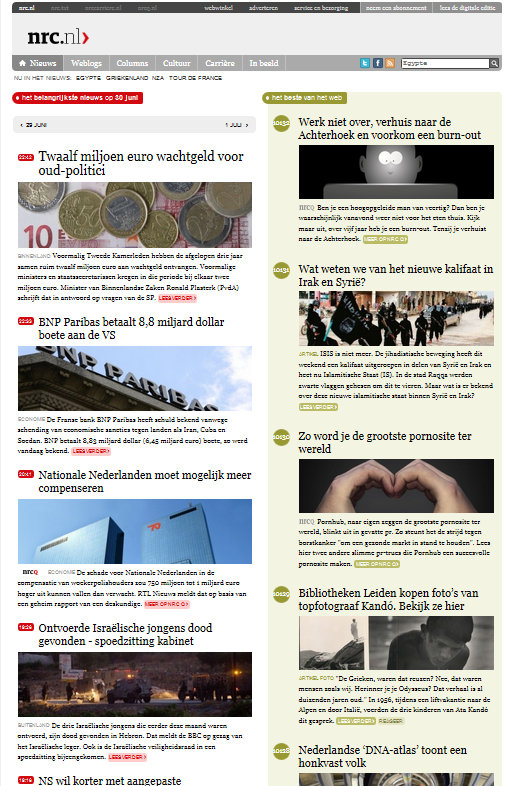
\includegraphics[height = 10cm]{June30}
	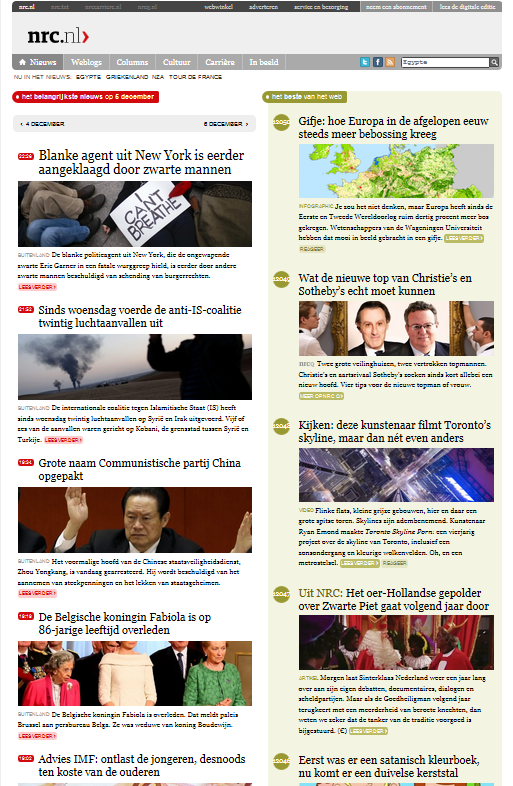
\includegraphics[height=10cm]{December5}
\end{figure}

These tweets were initially in JSON format, but were pre-processed into a utf-8 text file containing only the tweet id and the text. This conversion should not have impacted any character in Dutch, though it was noted that some emoticons were not preserved correctly in this format. 
As the language models were built over words, some linguistic preprocessing took place, namely that the text was converted to lowercase, punctuation was split from the words that it followed and treated as a separate token (though consecutive punctuation marks were considered as candidates for emoticons, and thus not split), and usernames and URLs were masked with a generic symbol. The use of hashtags was optional for the clustering scripts, and later we will see how this affected the model.

\subsection{Advantages of selecting micro-blogs as documents for topic-modelling}
Due to the short nature of micro-blogs and SMS messages, particularly twitter (which is notorious for the well-known cap at 140 characters), some additional assumptions can be made which ease the parameters required for topic-modelling:
Firstly, that each tweet addresses one topic, and also that long-distance dependencies are less likely to occur.
Secondly, many elements of a tweet, particularly hashtags, function as unigrams – though there are conventions that they often occur at the end of tweets, there is no grammar describing the particular order that they occur in (though this would be an interesting topic for future work.)  Thus, a bag of words model is particularly appropriate for these elements.
Thirdly, micro-blogs are often characterised by their use of non-standard language variants, such as alternative spellings, idiomatic or dialectal language, or use of slang. Similarly, the new expressions and words are often coined on the platform itself. These expressions may be topic-specific, and can uniquely be modelled on a corpus of micro-blogs, rather than a more traditional news corpus or web-crawl. This also requires that the models be updated online, so that the topics can shift with the discourse on the platform, and so that any newly-coined phrases are not out of vocabulary.

\subsection{Disadvantages of selecting micro-blogs as documents for topic-modelling}
As the micro-blogs are themselves quite short, many approaches combine the tweets of a certain topic with a supplementary corpus, in order to ensure that all words related to a topic are collected in the language model (cf. Kireyer et al 2009).
Additionally, given that the content is unedited and often produced quickly on mobile devices, misspellings or typographical errors are more likely to occur in this modality (). Though metrics such as the Levenshtein distance exist, which can tell us how orthographically close to another word a candidate is, these cannot be efficiently applied within this application of topic models. Thus such words are labelled as 'unseen' and given some smoothed probability.
The amount of tweets collected made the processing of the topic-models particularly difficult, suggesting two possible options: 1) Select a subsection of documents for each day, and model topic-document dependences over a longer period of time, allowing the observation of changes in the topic mixes over time (eg whether users post more about movies/sports on the weekend), though risking that a fixed number of topic models may mean that the topics are broader, or 2) take the full twitter stream collected over one day, hopefully generating more dense representations of the topics modelled. 
Intuitively, this second approach should result in more coherent topics, as we can presume that the range of topics discussed on one day on a micro-blogging platform is smaller than that over several days, thus this second approach was selected. Hopefully this means that more related words are captured, decreasing the number of OOV items encountered at testing.
With such large amounts of data being continuously generated by the users, it is important to maintain a model that does not infinitely grow and affect performance. Lau, Collier and Baldwin () offer a solution, taking time-slices from the micro-blog stream and recalculating their topic models based on this new training data. The size of the model is also a concern on this approach, as the motivation of this approach is to provide a language model that could be applied on a smart phone, and therefore must be limited in size. This is a motivation for the exploration of the cache.

\FloatBarrier
\subsection{Data used for topic exploration}
\begin{table}
	\begin{tabular}{|c|c|c|}
	\hline
	& June 30 2014 & 5 December 2014 \\
	\hline
	Number of tweets in corpus & 1,070,957 & 826,245 \\
	Number of unique users captured & 262,846 & 205,146 \\ % cut -f2 iut.normalday.txt | sort | uniq| wc -l
	Train/Dev/Test & 856,767 / 107,095 / 107,095 & 660,997 / 82,624 / 82,624 \\
	Average tweet length & 0 & 0\\
	\hline
	\end{tabular}
\caption{Tweets used for topic exploration by day}
\end{table} 

Two options were considered for the splitting of the data – due to the nature of the cache, the testing data should be contiguous and in order, so that all the appropriate terms are captured and available for the next item to be tested. Though a perl script was available to split the data by line, this would invalidate the cache option, as later micro-blogs would already be included in the topic model.
The pitfall of this approach, is that the topic mixtures are likely to change over the course of the day – that is, the final 10\% of the data occurred late at night, where the nature of the tweets may be very different from that in the morning and afternoon, on which the models were trained.  % [PUT HERE A DIAGRAM OF HOW THE TOPIX MIXTURES VARY!]
Another option for the split would be to take contiguous tweets from the end of the day, as this current training setup means that the use of cache is less useful. However, this means that the topic distribution over the time of day would have an effect.


\section {Topic models used: Theoretical summaries}
The topic models selected in this paper were chosen so as to represent a range of topic-modelling strategies, from outdated strategies from the later 1990s to popular current strategies. Whilst some of the older approaches have clearly been superseded, they still have value in that the efficiency required due to hardware constraints at their time of inception is a valuable feature for platforms such as twitter which handle so much new information that efficient approaches are necessary. 
Additionally, an inspiration for this paper is the work of Iyer and Ostendorf (1999), who used a two-step process to build topic models over North American Business Corpus (NAB) documents in an attempt to improve language model performance for speech recognition  by modelling sentence mixtures over different topics. The assumtion that one topic holds for one sentence is extrapolated in this paper to apply to one micro-blog posting, thus in the following section, the terms \textit{sentence} and \textit{document} are used interchangeably.

\subsection{k-Means with tf.idf}
Although the k-Means approach was described initially by MacQueen (1967)(cite), it has more recently been applied to document clustering using tf.idf scores, and has also been applied to document cluster since the 1980s (list papers). While variants such as \textit{Scatter/Gather} (cite Dougless R Cutting) and differing initialisations (cite Bradley and Fayyad Refining Initial points ...), the standard implementation is followed in this approach:
\begin{enumerate}
	\item DESCRIBE AS PROGRAMMING
\end{enumerate}

\subsection{Iyer and Ostendorf 1999: Approach 1 - Agglommerative clustering with tf.idf-like score} \label{sec:IO1}
% yields flat clusters per topic
Iyer and Ostendorf's 1999 approach interpolates individual topic-models and a global language model's score over each sentence, presuming that the topic-mixture in a sentence stays constant. To train these topic models, a two-step model-building process is applied. The first step builds hard clusters using an agglomerative clustering technique, with the stopping criterion being when the desired number of clusters is reached. The similarity measure used to merge clusters operated over the shared vocabulary of the clusters, and utilsed inverse document frequency measures, as well as normalising for the size of clusters.
\begin{equation}
S_{ij} = \sum_{w \in A_i \cap A_j}  \frac{N_{ij}}{|A^w|} \times \frac{1}{|A_i||A_j|}
\end{equation}
with $A_i$ and $A_j$ being the number of unique words in the articles, and $A^w$ being the number of documents containing the word. The normalisation constant $N_{ij}$ was necessary to prevent one large cluster accumulating all new documents, by virtue of having a larger shared vocabulary which contributed to the similarity score (confirmed by testing), and was calculated as 
\begin{equation}
N_{ij} = \sqrt{\frac{N_i+N_j}{N_i \times N_j}}
\end{equation}
This approach uses unigrams, and no smoothing is applied as the score is only calculated over the intersection of the vocabularies of the clusters being compared.
% unigram, counts only (no LM required)


\subsection{Iyer and Ostendorf 1999: Approach 2 - Iterative re-estimation of topic-models with EM}
% yields trigram smoothed LM per topic
 % trigram with Witten-Bell
From the hard clusters created in the first step (see sections \ref{sec:IO1}, \ref{sec:goodman}), initial n-gram language models are constructed. The original paper utilised a trigram language model with Witten-Bell smoothing.

\subsection{Gildea and Hoffman 1999: Topic-based Language Models with EM}
% yields unigram LM pertopic
% unigram into tdm (unigrams make topic, one-word history gives topic, topic gives word.)
This approach was tested over the Wall Street Journal and TDT-1 corpora and demonstrated that the addition of a topic modell to standard unigram/bigram/trigram models resulted in a large decrease in perpexity. However, the topic model's unigram nature means that if it is not interpolated with standard n-gram data, the word probability is only conditioned upon the topic, and the topic is only conditioned on the history:
$$P(w|h) = \sum_{t}P(w|t)P(t|h)$$,
thus it functions effectively like a bag-of-words model. However, this may actually suit the nature of \textit{hashtags} and their use on social-media, and lead to less data sparsity than, say, a trigram approach.

Withthe number of topics $t$ predetermined, the parameters are randomly initialised such that each word is given a random assignment to a topic (summing to 1 for each topic like a normal LM), and a topic mixture (summing to 1) is assigned to a document. For example, $d_1$ may receive the following topic assignments: $d_1: \{t_1:0.4, t_2: 0.2. t_3: 0.2\}$.
The original paper used a modified E-step, but this approach followed the generic E-step
\begin{equation}
P^{(r)}(w|t) = \frac{P^{(r-1)}(w|t)P^{(r-1)}(t|d)}{\sum_{t'}P^{(r-1)}(w|t')P^{(r-1)}(t'|d)}
\end{equation}

and M-step
\begin{equation}
P^{r}(w|t) = \frac{\sum_{d}n(w,d)P^{(r)}(t|w,d)}{\sum_{w'}\sum_{d}n(w',d)P^{(r)}(t|w',d)}
\end{equation}
\begin{equation}
P^{r}(t|d) = \frac{\sum_{w}n(w,d)P^{(r)}(t|w,d)}{\sum_{t'}\sum_{w}n(w,d)P^{(r)}(t'|w,d)}
\end{equation}
stopping when ??? % WHEN DID MY IMPLEMENTATION STOP


\subsection{Goodman 2001: Simplified implementation of I\&O 1999: Minimizing unigram perplexity} \label{sec:goodman}
% yields flat clusters per topic
% When experimenting with the models, used Kneser-Ney smoothing.
Goodman's implementation of Iyer and Ostendorf's work used a different implementation, leveraging his previous work on finding clusters of words (IBM clustering) based in minimising the bigram perplexity within the clusters. Thus, the implementation for finding making the topic LMs was that of creating hard clusters by ``minimiz[ing] the sentence-cluster unigrm perplexities''. This aimed to maximise the value
$$\prod_{i=1}^{N}P(w_i|s(i))$$
that is, the product of every word when given the topic (sentence) probability of that word, using unigrams. Language models were then trained on these clusters, and there was no secondary EM step to adjust the probabilities.

\FloatBarrier
\subsection{Bellagarda 2000: Latent Semantic Analysis}

This utilises singular value decomposition:
$$W \approx USV^T $$
\begin{figure}
	\caption{Excerpt of Fig.1 from Bellagarda illustrating Singular Value Decomposition}
	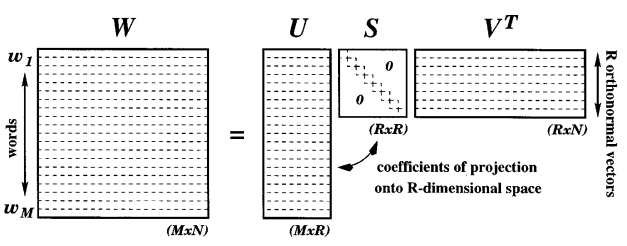
\includegraphics[width=\textwidth]{Bellagarda_fig1_cropped}
\end{figure}

\subsection{Blei et al 2003: Latent Dirichlet Allocation}
$$$$


% Summarise theoretical findings in a table
\begin{table}
	\begin{tabular}{|c|c|c|c|} % Name, Hard, Hierarchical/Flat, Soft, Flat, 
	\hline
	Name 		& Hard 	& Hier./ Flat 	& Soft \\
	\hline
	I\&O1 	& $\bullet$  	& Hier.		&\\ 
	I\&O2 	& 		& 			&\\
	G\&H 		& 		& 			&\\
	Goodman	& $\bullet$	& Flat			& \\
	\hline
	\end{tabular}
\caption{Summary of the methods explored}
\end{table}



\end{document}


